\documentclass{cup-pan}
\usepackage{blindtext}
\usepackage{xcolor}
\usepackage{import}

\import{dev/}{packages}

\import{dev/}{commands}

\title{E-learning Recommender Systems Based on
Deep Learning }

\author[ ]{Ikram Damri*, Mohamed Biniz}

\affil[      ]{Laboratory of Innovation in Mathematics, Applications and Information Technology,}
\affil[ ]{Polydisciplinary Faculty, Sultan Moulay Slimane University, Beni Mellal, Morocco.}

\affil[  ]{}
\affil[ ]{*Corresponding author E-mail: \url{ikram.damri@usms.ac.ma}}

%% Corresponding author
\corrauthor{Author One}

%% Abbreviated author list for the running footer

\addbibresource{refs.bib}

\begin{document}

\maketitle

\begin{abstract}
The digital age has resulted in an overwhelming amount of information and choices, leading to decision exhaustion and suboptimal decisions for users. Recommender systems have emerged as crucial tools to address this challenge by providing personalized recommendations and improving the decision-making process. This research specifically focuses on the significance of recommender systems in e-learning. In the e-learning context, these systems offer substantial benefits to learners and educational institutions by suggesting relevant courses, materials, and resources based on learner preferences and goals. They also enable adaptive learning paths, foster social learning, and provide valuable data for optimizing course offerings and instructional design. Additionally, recommender systems help mitigate overcrowding issues in e-learning platforms by efficiently guiding learners through content discovery. The project explores various approaches, including deep learning techniques like deep collaborative filtering and restricted Boltzmann machines, to analyze user behavior and generate accurate recommendations. By continuously learning and adapting to user feedback, recommender systems contribute to a personalized, efficient, and engaging e-learning experience. The project presents further contributions and findings to enhance the discussed approaches.

\keywords{recommender systems; deep learning; rating; collaborative filtering; personalized recommendations; e-learning; restricted Boltzmann machine.}
\end{abstract}

\section{Introduction}
\label{sec:overview}
\paragraph{}
Among the challenges users face in the digital age are due to the overwhelming amount of information and choices available. Recommender systems have emerged as essential tools to address this challenge by providing personalized recommendations in various industries \cite{1, 2}, such as e-commerce, entertainment, and e-learning. These systems enhance the decision-making process, reduce cognitive load, and increase user engagement and satisfaction. This paper specifically focuses on the importance of recommender systems in the e-learning field, where they offer personalized learning experiences and adaptive learning paths, and support lifelong learning. Additionally, recommender systems play a vital role in addressing overcrowding issues in e-learning platforms by providing tailored recommendations that match learners' interests and proficiency levels. The paper also highlights the use of sophisticated algorithms and data analysis techniques in these systems to generate accurate and evolving personalized recommendations.
\paragraph{}
In the e-learning field, recommender systems offer substantial benefits to both learners and educational institutions \cite{3}. They provide a personalized learning experience by suggesting relevant courses, materials, and resources, and facilitate adaptive learning paths based on learners' progress and performance. These personalized recommendations enhance engagement, motivation, and satisfaction within e-learning platforms. Additionally, recommender systems support lifelong learning by recommending relevant courses for continuous skill development and fostering social learning through study groups and peer activities. From an institutional perspective, they provide valuable data to optimize course offerings and improve curriculum design \cite{3}.
\paragraph{}
Furthermore, recommender systems play a vital role in addressing overcrowding issues in e-learning platforms by offering tailored recommendations that match learners' interests and proficiency levels \cite{4}. They streamline information overload, enhance engagement, and ensure relevant content access, leading to a smoother learning experience in overcrowded environments.
\paragraph{}
All in all, recommender systems have transformed decision-making processes in various industries and proved their significance in offering personalized recommendations, enhancing user experiences, and tackling overcrowding challenges.

\section{Literature Review}
\label{sec:overview}
\paragraph{}
Collaborative filtering (CF) is a commonly used technique that identifies similarities between users based on their past behavior and suggests items that similar users have liked or purchased \cite{5}. It is divided into two types: User-based and item-based.
Collaborative filtering algorithms are widely used in e-learning recommender systems to analyze user behavior and preferences, identify patterns of similarity between learners, and then make recommendations. For instance, if Learner A has a history of performing well on the same
types of exercises as Learner B, and Learner B has recently completed a new exercise successfully, then Learner A is likely to perform well on that exercise as well. This approach works well for datasets with a large number of learners and a relatively small number of educational resources.
\paragraph{}
User-based and item-based CF approaches have some limitations that can affect their accuracy in making recommendations. One of the main challenges is the data sparsity problem \cite{6}, where the algorithms struggle to build a relationship model between users and items due to the limited data available. This can result in inaccurate recommendations or predictions.
\\
Another limitation is the early rater problem \cite{7}, where new items or users with limited ratings can be difficult to predict accurately. These limitations have been studied extensively in the literature, and researchers have proposed various techniques to address them.
\paragraph{}
Due to these limitations, the model-based approaches are introduced. There are many well-established model-based approaches, among which the matrix factorisation (MF) approach is widely used. It works by making an assumption that there exist some latent features which explain user preferences. It leads to uncover these latent features which can afterward be used to predict items for a user more accurately \cite{8}.
\paragraph{}
The autoencoders are also widely used in the field of recommenders. Autoencoders are often faster in recommender systems because they can operate directly on the sparse input data matrix that is common in recommendation tasks \cite{9}. In contrast, traditional methods like matrix factorization require converting the sparse matrix to a dense matrix, which can be computationally expensive for large datasets. They can also be more efficient in terms of memory usage since they can use smaller embedding dimensions to represent the input data compared to matrix factorization. This can be particularly important in scenarios where the input data has high dimensionality \cite{10}.
\paragraph{}
In this context, the autoencoder is used in many recommenders since it is a basic intuition when it comes to the machine and deep learning of the day. Among the works we cite is once again the movie dataset used to train it in the autoerc model in \cite{11}
\paragraph{}
A stochastic generative artificial neural network, Restricted Boltzmann Machine (RBM), is also used since it can learn a probability distribution over its set of inputs \cite{12}.
\paragraph{}

Both autoencoders and RBMs have an encoder part that maps the input data to a hidden representation, and a decoder part that maps the hidden representation back to the input space.
\\\\
In an autoencoder, the encoder typically consists of one or more fully connected layers that reduce the input data into a lower-dimensional hidden representation, while the decoder consists of one or more fully connected layers that reconstruct the input data from the hidden representation.
\\\\
In an RBM, the encoder is the set of hidden units, which take the input data and produce a hidden representation. The decoder is the set of visible units, which generate the reconstructed input data from the hidden representation.

\section{Dataset}
\label{sec:overview}
\paragraph{}
Through this project, we chose to work with the most recent Coursera Courses Dataset.
The Coursera Courses Dataset 2021 is a publicly available dataset containing information on tens of thousands of courses offered on the Coursera platform as of 2021. The dataset includes details on courses in 9 columns, including User ID, Course ID, Course Rating, Course Name, University, Difficulty Level, Description, and other relevant information.
\\
Here is a description of the columns:
\begin{enumerate}
  \item \textbf{User ID}: This column contains a unique identifier for each user who has rated a course on the Coursera platform.
  \vspace{0.3cm}
  \item \textbf{Course ID}: This column contains a unique identifier for each course offered on the Coursera platform.
  \vspace{0.3cm}
  \item \textbf{Course Rating}: This column contains the rating given to the course by the user, on a scale of 1 to 5.
  \vspace{0.3cm}
  \item \textbf{Course Name}: This column contains the name of the course offered on the Coursera platform.
  \vspace{0.3cm}
  \item \textbf{University}: This column contains the name of the university or institution that offers the course on the Coursera platform.
  \vspace{0.3cm}
  \item \textbf{Difficulty Level}: This column contains the difficulty level of the course, as rated by the university or institution offering the course.
  \vspace{0.3cm}
  \item \textbf{Course URL}: This column contains the URL of the course on the Coursera platform.
  \vspace{0.3cm}
  \item \textbf{Course Description}: This column contains a brief description of the course and what it covers.
  \vspace{0.3cm}
  \item \textbf{Skills}: This column contains a list of skills that are taught or covered in the course.
\end{enumerate}
\paragraph{}
The dataset is medium-sized, with a shape of (3522, 9), indicating that it likely contains a lot of valuable information for researchers, educators, and data analysts interested in exploring trends and patterns in online education.

And here is the graphical visualization of the dataset using a bar plot of the \textit{'Course Rating'} column since it is the column associated to prediction. the \textit{Count} represents the count or frequency of each unique value in the 'Course Rating' column.

\begin{center}
  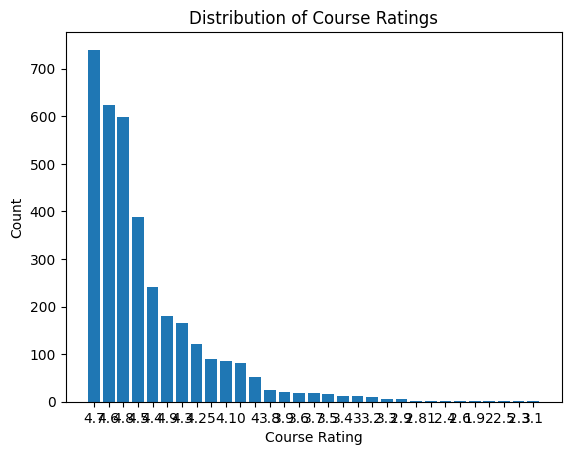
\includegraphics[width=350px]{imgs/figures/25.png}
  \captionof{figure}{Dataset visualization with respect to 'Course Rating' main column with bar plot.}
  \vspace*{.1cm}
\end{center}



\section{Contributions and Findings}
\label{sec:overview}

\paragraph{}
In this section, we delve into the exploration of matrix factorization and Restricted Boltzmann Machines as powerful techniques within the field of personalized recommender systems.
Specifically, we investigate their application and impact within the e-learning domain platforms, in addition, we will try to make a hybrid model as a chance for more potential models.
\subsection{Candidate Re-ranking}
\label{sec:overview}
\paragraph{}
Recommender systems can help correlate information and recommend personalized services to users as a general information filtering tool. However, contextual factors significantly affect user behavior, especially in the Internet of Things, which brings difficulties to modelling user preferences \cite{13}.
\paragraph{}
The idea behind candidate re-rank is to recommend the recommendation, which means looking at the top N recommended courses in a previous recommendation using an algorithm. So the basic idea of this method is that the items in the new ranked list should be ranked higher than the initial ranking \cite{14}. In our project, we used matrix factorization, and then based on some added features, we apply the re-ranking. In our case, we will sort the recommendation based on the "Difficulty Level" feature according to our datatset.
\begin{center}
  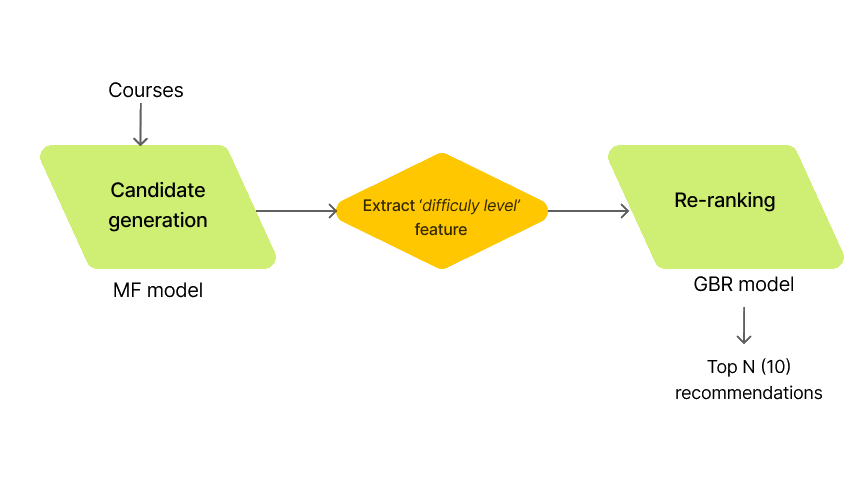
\includegraphics[width=350px]{imgs/figures/17_2new.png}
  \captionof{figure}{recommender candidate generation/rerank technique used in this project.}
  \vspace{.1cm}
\end{center}
\subsection{Improved Restricted Boltzmann Machine}
Since the input to the RBM will is used as one hot encoded rating, then we will need to use it from scikit-learn library, however it is a burden to make it ourselves since it does not accept float numbers as input. It is specifically designed to handle categorical features, which are typically represented as strings or integers.
\\
Also, the OneHotEncoder in scikit-learn expects a 2-dimensional (sample, feature) input and returns 2-dimensional as output which is not our case, because we have 3-dimensional shape (sample, feature, class).
\paragraph{}
Well it's that we have to do all this one hot encoding and NumPy. Ideally, that would be done in Tensorflow. And what really makes it inefficient is that we have to do this on every single batch. So what if we just did it on the entire dataset all at once. Then we wouldn't have to do it on every batch we could just pass in the 100 encoded versions into the RBM model directly.
\paragraph{}
In tensor flow, we create the 3D mask which actually just repeats the 2D mask k times instead of hardcoding a function for it. Finally converting probabilities into ratings is just a dot product, so we can easily include it in the RBM model. This is going to make the code a little more compact and it'll also run much faster.
\paragraph{}
Let's now get an idea about the results provided by the RBM model in coursera dataset.
\begin{center}
  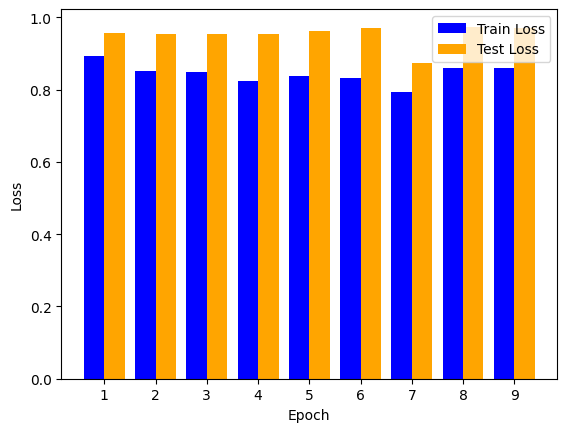
\includegraphics[width=350px]{imgs/figures/35.png}
  \captionof{figure}{RBM train/test bar chart results.}
  \vspace{.1cm}
\end{center}
\vspace*{.3cm}
\begin{center}
  \begin{tabular}{|c|c|c|}
    \hline 
    \textbf{Cost duration for previous RBM} & \textbf{Cost duration for new RBM} & \textbf{Percentage Difference}\\
    \hline 
    0:00:24.047864 & 0:00:01.790108 & 172.287\% \\
    0:00:23.600937 & 0:00:01.457430 & 176.735\% \\
    0:00:25.874191 & 0:00:01.449281 & 178.783\% \\
    0:00:24.282049 & 0:00:01.258427 & 180.291\% \\
    0:00:24.237422 & 0:00:01.250107 & 180.381\% \\
    0:00:31.981618 & 0:00:01.256549 & 184.878\% \\
    0:00:25.871161 & 0:00:01.582297 & 176.946\% \\
    0:00:27.334085 & 0:00:01.268047 & 182.266\% \\
    0:00:25.841910 & 0:00:01.260135 & 181.402\% \\
    0:00:25.927237 & 0:00:01.254201 & 181.543\% \\
    \hline
  \end{tabular}
  \captionof{table}{Cost duration for previous RBM vs. Cost duration for new RBM.}
\end{center}

We calculate the Percentage Difference where: 
\\
\textit{Percentage Difference} = $\frac{\left|V_1-V_2\right|}{\left(V_1+V_2\right)/{2}} \times 100$
Where:
\\
\begin{itemize}
  \item $V_1$: is the cost duration for previous RBM.
  \item $V_2$: the cost duration for new RBM.
\end{itemize}

It is clearly that the MSE cost duration is improved from the old version compared to the new one, by an average of 181.6532\%, which has a huge impact especially when we are dealing with a millions of datasets in the real world. 
\\I
In addition, the old RBM model is swinging between 24 seconds up to 31 seconds so it is unstable; however, the second model is stable as it stacks a 1 second duration.
\\
We also provide other metrics values like Hit Rate, Mean Absolute Error, Root Mean Square Error in the following table:

\begin{center}
  \begin{tabular}{||c|c|c|c|c||}
    \hline\hline 
    \textbf{Metric} & \textbf{MSE} & \textbf{MAE} & \textbf{RMSE} & \textbf{HR} \\
    \hline 
    \textbf{Value} & 0.9731242420682709 &  0.024747825710443382 & 0.9864705986841528 & 0.07525 \\
    \hline\hline
  \end{tabular}  
  \captionof{table}{Error measures values by metrics}
\end{center}

\subsection{Hybrid RBM and Autorec model}
\label{sec:overview}
\paragraph{}
The Hybrid Model capitalizes on the individual advantages of RBMs and Autoencoders, resulting in improved performance across various tasks, with a particular emphasis on recommendation systems. To grasp the importance of this Hybrid Model, it is essential to explore the underlying algorithms and their collective contributions to the model's overall functionality.

\paragraph{}
The Hybrid Model combines the power of RBMs and Autoencoders by utilizing the RBM's ability to capture complex dependencies and the Autoencoder's capacity for efficient dimensionality reduction and reconstruction. During training, the RBM and Autoencoder are trained iteratively, with the RBM providing the initial feature representation for the Autoencoder. This joint training process allows the model to leverage the strengths of both algorithms and achieve enhanced performance compared to using either algorithm individually.
\paragraph{}
This model has been successfully applied to recommendation systems, where RBMs capture user-item preferences and Autoencoders provide efficient dimensionality reduction for recommendation tasks. Therefore, the following results are achieved.

\begin{center}
  \begin{tabular}{||c|c|c|c|c||}
    \hline\hline 
    \textbf{hybrid MSE} & \textbf{hybrid RMSE} \\
    \hline 
    0.9380617395786907 &  0.9685358741826193  \\
    \hline\hline
  \end{tabular}  
  \captionof{table}{Error measures values by MSE/RMSE metrics}
\end{center}

\section{Evaluation and Discussion}
\label{sec:overview}
\paragraph{}
\subsection{Evaluation Metrics}
\paragraph{}
Evaluation metrics in recommender systems play a crucial role in assessing the performance and effectiveness of recommendation algorithms. These metrics are specifically designed to measure the quality, accuracy, and relevance of recommendations provided by the system.
\paragraph{}
Common evaluation metrics in recommender systems take into account various factors such as relevance, ranking, and user interactions to capture the performance of recommender algorithms accurately.
\paragraph{}
We use the following evaluation metrics to measure the quality of the models in discussion.
\\
Let's first put notations in order to keep the metrics formulas short.
\begin{itemize}
  \item $r_{ui}$: It represents the actual or observed rating given by user $u$ for item $i$. This is the true rating that we want to compare with the predicted rating.
  \item $\hat{r}_{ui}$: It represents the predicted rating for user $u$ and item $i$ provided by the recommender system.
  \item $|\hat{R}|$: It represents the cardinality or the total number of predicted ratings $\hat{r}_{ui}$ in the set $\hat{R}$. It denotes the number of ratings for which predictions were made.
  \item $\sum_{\hat{r}{ui} \in \hat{R}}$: This symbol denotes the summation over all predicted ratings $\hat{r}{ui}$ in the set $\hat{R}$. It indicates that we are summing the following expression for each predicted rating.
\end{itemize}
\paragraph{}
\noindent
Now, we can easily refer these notations to the following metrics:
\\
\begin{itemize}
  \item RMSE: Root Mean Squared Error. RMSE provides a numerical measure of the prediction error, allowing the performance of different recommendation algorithms or models to be compared. A lower RMSE indicates better accuracy in predicting user preferences and can be used as a benchmark for evaluating and optimizing recommender systems.
  \begin{align}
  \mathrm{RMSE}=\sqrt{\frac{1}{|\hat{R}|} \sum_{\hat{r}_{u i} \in \hat{R}}\left(r_{u i}-\hat{r}_{u i}\right)^2}
  \end{align}
  
  \item MSE: Mean Squared Error is another commonly used evaluation metric in recommender systems, similar to RMSE. It is a measure of the average squared difference between the predicted ratings or scores and the actual ratings provided by users. Lower values mean better accuracy.
  \begin{align}
  \mathrm{MSE}=\frac{1}{|\hat{R}|} \sum_{\hat{r}_{u i} \in \hat{R}}\left(r_{u i}-\hat{r}_{u i}\right)^2
  \end{align}
  \item MAE: Mean Absolute Error. A commonly used evaluation metric in recommender systems. It measures the average absolute difference between the predicted ratings or scores and the actual ratings provided by users. Lower values mean better accuracy.
  \begin{align}
  \mathrm{MAE}=\frac{1}{|\hat{R}|} \sum_{\hat{r}_{u i} \in \hat{R}}\left|r_{u i}-\hat{r}_{u i}\right|
  \end{align}
  \item HR: Hit Rate. Measures the success rate of the recommendations in terms of whether the recommended items were relevant or clicked on by the users. Briefly, the hit rate is how often we are able to recommend a left-out rating. Higher value is better.
  \begin{align}
  HR = \text{(Number of successful recommendations) / (Total number of recommendations)}
  \end{align}

  \item ARHR: Average Reciprocal Hit Rank. is an evaluation metric used in recommender systems to measure the effectiveness of the system in terms of ranking relevant items higher in the recommendation list. The formula for ARHR is as follows:
  \begin{align}
    ARHR = \text{(1 / Rank of the first relevant item) / (Total number of recommendations)}
  \end{align}
\end{itemize}
\paragraph{}
The paper tried the Matrix factorization on Coursera Dataset of 2017, and the approches used are KNN, SVD, and Neural collaborative filtering. The model that we implement in this project based on matrix factorization can combine between NCF and SVD as discussed in \ref{sec:section3}, since it is a model developed from the limitation of CF and uses SVD, and the more important is that is neural network. Briefly the folloSE: Root Mean Squared Error. wing results are found.
\begin{center} 
  \begin{tabular}{||c|c||c|c|c|c|c||}
    \hline\hline 
    \multicolumn{2}{||c||}{\textbf{Coursera Reviews Approach}} & \multicolumn{5}{c||}{\textbf{Metrics}} \\
    \hline
    \textbf{Technique} & \textbf{Description} & \textbf{MSE} & \textbf{MAE} & \textbf{RMSE} & \textbf{HR} & \textbf{ARHR} \\
    \hline 
    SVD  & basic (MF) & - & 0.0260 & - & 0.7992 & 0.1229 \\
    NCF & ANN based & - & 0.0175 & - & 0.9371 & 0.1441 \\
    \hline\hline
    \multicolumn{2}{||c||}{\textbf{Our Coursera Ratings Approach}} & \multicolumn{5}{c||}{\textbf{Metrics}} \\
    \hline
    MF & basic (SVD) & 0.1219 & 0.3127 & 0.3812 & 0.6894 & 0.1456 \\
    MF & ANN based & 0.1269 & 0.2291 & 0.3562 & 0.226 & 0.326 \\
    \hline\hline
  \end{tabular}
  \captionof{table}{Performance metrics for CF based model on Coursera reviews dataset project and our ratings Coursera dataset.}
\end{center}
\paragraph{}
Taking in consideration that the review dataset is much bigger than our rating dataset, make some sense when we compare the MAE which performs better in the first one due to the added bunch of information and learning the new patterns. Unfortunately, the paper doesn't present the way the dataset is preprocessed to get an idea and might be a cause to implement our dataset using it for better comparaison.
\paragraph{}
However, a new metric key may get us into more comparaison between the approches. The paper approach has a higher HR value, indicating a higher probability of including at least one relevant item, while our approach has a higher ARHR value, indicating better ranking of the relevant items on average.
\paragraph{}
In other hand, HR does not take into account the order or ranking of the recommended items. Therefore, in this comparison, the second approach outperforms the first one in terms of ARHR, suggesting that it provides better recommendations with a higher likelihood of including relevant items and higher ranking of those relevant items within the recommendation list.
\subsection{Results Validation}
\paragraph{}
In order to validate the performance of our models, we suggest making use of real-world datasets of the most common and international companies, including industry leaders such as Amazon and Netflix then the famous MovieLens dataset which is commonly used for testing recommender systems models to make sure of their evaluation.

\subsubsection{Netflix Dataset}
\paragraph{}
Netflix dataset is among the famous one that works as a recommender
system since Netflix is among the huge streaming companies that developed their
technical content over time.
\\ 
Here we have a study at the Polytechnic University of Madrid (UPM) \cite{15} where the researchers improve the MF in Netflix model, also, we have a project \cite{16} done by a Master student in Business Analytics at University of California, Davis (UC Davis), United States, in which we will make the comparison.

\begin{center} 
  \begin{tabular}{||c||c|c|c| c||}
    \hline\hline 
    \textbf{MF} & \multicolumn{1}{c}{\textbf{}} & \multicolumn{3}{c||}{\hspace{-1.5cm}\textbf{Metrics}} \\
    \hline\hline 
  
    
    \multicolumn{1}{||c||}{\textbf{Approaches}} & \textbf{MSE} & \textbf{MAE} & \textbf{RMSE} & \textbf{HR}\\
    \hline 
    UC Davis project & - & 0.7882 & 0.9855 & -\\
    UPM project & - & 0.60 & - & - \\
    Our project & 0.5888 & 0.6001 & 0.7632 & 0.092\\
    \hline\hline
  \end{tabular}
  \captionof{table}{Performance metrics for MF based model on Netflix dataset, in the cited studies vs. our model.}
\end{center}

The major results preference is attributed to our model, moreover, the added value of MSE and HR emphasizes the better quality of our model.
\paragraph{}
We also provide RBM results since RBM is seen as the main improved algorithm in this project, and it really needs an evaluation in real word dataset to prove its improvement. Here we recall the famous research for RBM in RBM for CF \cite{17} for University of Toronto which has been cited by many other bleeding edge researches (view \cite{17}).
\begin{center} 
  \begin{tabular}{||c||c||}
    \hline\hline
    \textbf{RBM} & \textbf{Metrics} \\
    \hline\hline
    \textbf{Approaches} & \textbf{RMSE} \\
    \hline
    University of Toronto project & 0.99 \\
    Our project & 0.86 \\
    \hline\hline
    \end{tabular}
  \captionof{table}{Performance metrics for RBM based model on Netflix dataset, in the RBM for CF vs. our model for RBM for CF.}
\end{center}

\subsubsection{Amazon Dataset}
E-commerce websites utilizes some very strong recommender systems, however and according too the large dataset, it is needed each time to update models, and of course make some new studies to try to improve the recommenders models. In this context, we cite some studies that worked on the Amazon datasets \cite{18}, starting from the study of a professional engineer \cite{19} with overall 11 years of total experience in the field of data science, analytics and Automation and then worked recently as a Data Scientist at Kramp. And the study of \cite{20} at the University of California (UC) San Diego, that worked on the same dataset, which is a good commun point to make efficient results in term of comparaison. Here are the following results.


\begin{center} 
  \begin{tabular}{||c||c|c|c|c||}
    \hline\hline 
    \textbf{} & \multicolumn{1}{c}{\textbf{}} & \multicolumn{3}{c||}{\hspace{-1.5cm}\textbf{Metrics}} \\
    \hline\hline 
    \multicolumn{1}{||c||}{\textbf{Approaches}} & \textbf{MSE} & \textbf{MAE} & \textbf{RMSE} & \textbf{HR} \\
    \hline 
    UC San Diego & - & 1.58 & 1.63 & - \\
    Kramp engineer model & - & - & 1.3436 & - \\
    Our project & 0.7621 & 0.6629 & 0.8730 & 0.1847 \\
    \hline\hline
  \end{tabular}
  \captionof{table}{Performance metrics for MF based model on Amazon dataset, in the cited studies vs. our model.}
\end{center}

Actually, there is a huge difference between our model and the Amazon evaluation by the cited studies in terms of MAE and RMSE, but especially when we added other metrics to confirm this good performance (MAE and HR)

\subsubsection{MovieLens Dataset}
In this subsection, we will get a deep comparaison between our model and the real world datasets. First we will try the \textit{Movielens} dataset, which is a very famous dataset special for testing recommenders systems models since 1995; and effectively, it was used and is still used by many researches since it contains a large amount of data and growths by year. In this context, we will evaluate our model according to this dataset and use projects in different model implementations.
\paragraph{}
For a start, we cite this paper\cite{21} that tries SVD or, in other word, Matrix factorization with two different versions of Movielens dataset, the old one and newest. and as expected the old version gives remarkable lower RMSE results \textit{(0.9908)} since it doesn't contains so much information to help learning hidden patterns by the model. Here are the following results of the paper compared with our model.
\begin{center} 
  \begin{tabular}{|c|c||c|c|c|c|c||}
    \hline\hline 
    \multicolumn{2}{|c||}{\textbf{Matrix Factorization}} & \multicolumn{3}{c|}{\textbf{Learning Rate}} \\
    \hline
    \textbf{Approach} & \textbf{Metric} & \textbf{0.001} & \textbf{0.0001} & \textbf{0.06}\\
    \hline
    Paper MF model  & \multirow{2}{*}{RMSE} & 0.9096 & 0.9807 & - \\
    Our Project MF model &  & 0.8923 & 0.9789 & 0.8642 \\
    \hline
    \hline
    \multirow{4}{*}{Our Project MF model} & MSE & 0.7962 & 0.9582 & 0.5243 \\
    & MAE & 0.6894 & 0.7701 & 0.5542 \\
    & HR & 0.1569 & 0.0481 & 0.0682 \\
    & ARHR & 0.0467 & 0.0143 & 0.0391 \\
    \hline\hline
  \end{tabular}
  \captionof{table}{Performance metrics for MF based model on Movielens dataset, in the study \cite{21} vs. our model.}
\end{center}


It is noticeable that the increase of learning rate has an important impact on the results in all projects, especially, when modifying learning rate in our model to 0.06 which is, in fact, our original rate. However regardless of the learning rate, it is remarkable that our model performs better than the other project; as it has lower RMSE, but also a reasonable MSE compared to the accorded RMSE and an a lower MAE. We also reinforce its effectiveness using the HR and ARHR, and indeed, their values are higher.
\paragraph{}
We also provide RBM results on Movielens dataset as it can confirms the effectiveness of our project models, especially when dealing with this dataset for trying recommendation performance. In this context, we use the most recent studies for comparaison with the same dataset, and we choose the article Unsupervised Boltzmann machine-based time-aware recommendation system (UBMTR) \cite{22} since it shows some good results and improvement compared with the a famous implementations of other RBM models. We also provide \cite{23} since it is a recent research made also in comparaison with the (UBMTR) work to make a clear comparaison view.
\begin{center} 
  \begin{tabular}{||c||c|c|c|c||}
    \hline\hline 
    \textbf{RBM} & \multicolumn{1}{c}{\textbf{}} & \multicolumn{3}{c||}{\hspace{-1.5cm}\textbf{Metrics}} \\
    \hline\hline 
    \multicolumn{1}{||c||}{\textbf{Approaches}} & \textbf{MSE} & \textbf{MAE} & \textbf{RMSE} & \textbf{HR} \\
    \hline 
    UBMTR & 0.74 & - & 0.86 & - \\
    Yang et al. Approach & 0.848 & - & 0.921 & - \\
    Our project & 0.7405 & 0.029 & 0.851 & 0.0743 \\
    \hline\hline
  \end{tabular}
  \captionof{table}{Performance metrics for RBM based model on Movielens dataset, in the studies \cite{22, 23} vs. our model.}
\end{center}

According to this results, we found ourselves in a discussion between our model performance and UBMTR model, since they are clearly approximated, in our model there is a precision of 0.001 MSE, but unfortunately, it is not shown in the other study. Also, we have a better performance in terms of RMSE with, approximately, 0.01.


\paragraph{}
Trying Matrix Factorisation and Restricted Boltzmann Machine in these real-world datasets, makes results more realistic and reliable, and so since the Movielens dataset is made for testing recommender models performance, we decide to make a final step to clearly be undoubted about our models' performance. So we have a good MF and RBM model performance, why not evaluating the approach that makes good results in our contributions, which is the hybrid model of Autoencoder and RBM. First let's evaluate the autoencoder model, since there are many researches that worked with it as a recommender and this will make a new performance step to make evaluation.
\paragraph{}
We have the study of Biased autoencoder for collaborative filtering with temporal signals \cite{11}, the researchers focused on evaluating their models with RMSE metric on different Movielens dataset, and in this context, we will focus on the latest dataset since it make a big difference in the evaluation compared with the older versions of Movielens.
\\
We will also consider a study of Recommender System using Auto-encoders \cite{24} made by the junior programmer at the software company Lord of I in Dandenong, Australia. And what is interesting about this study is, luckily, measures different evaluation metrics, which makes the performance quality of the model more clear. Here are the results according to our study.

\begin{center} 
  \begin{tabular}{||c||c|c|c|c||}
    \hline\hline 
    \textbf{Autorec} & \multicolumn{1}{c}{\textbf{}} & \multicolumn{3}{c||}{\hspace{-1.5cm}\textbf{Metrics}} \\
    \hline\hline 
    \multicolumn{1}{||c||}{\textbf{Approaches}} & \textbf{MSE} & \textbf{MAE} & \textbf{RMSE} & \textbf{HR} \\
    \hline 
    Lord of IT programmer study & - & 1.6734 & 2.0340 & 0.0060 \\
    Autorec with temporal signals study & - & - & 0.8778  & - \\
    Our Autorec project & 0.7543 & 0.0200 & 0.8640 & 0.0331 \\
    \hline\hline
  \end{tabular}
  \captionof{table}{Performance metrics for Autoencoder based model on Movielens dataset, in the studies \cite{11, 24} vs. our model.}
\end{center}

\paragraph{}
Our model performs perfectly in the Autorec algorithm, especially it is better In contrast with other approaches in all metrics. Now, we can check our hybrid model performance in Movielens dataset.

\begin{center} 
  \begin{tabular}{||c||c|c|c||}
    \hline\hline 
    \textbf{Hybrid} & \multicolumn{1}{c}{\hspace{1.5cm}\textbf{Approaches}} & \multicolumn{1}{c||}{\hspace{-1.5cm}\textbf{}} \\
    \hline\hline 
    \multicolumn{1}{||c||}{\textbf{Metrics}} & \textbf{Hybrid Train} & \textbf{Hybrid Test} \\
    \hline 
    MSE & 0.5682 & 0.7416 \\
    RMSE & 0.7538 & 0.8612 \\
    \hline\hline
  \end{tabular}
  \captionof{table}{Performance metrics for Hybrid model (Autorec + RBM) based model on Movielens dataset.}
\end{center}
\paragraph{}
Since the results of the hybrid model seem a little ambiguous (no big difference between the non hybrid models), so let's make a comparaison to see the hidden differences.

\begin{center} 

  \begin{tabular}{||c||c|c|c||}
    \hline\hline
    \textbf{} & \multicolumn{2}{c||}{\textbf{Metrics}} & \multicolumn{1}{c||}{\textbf{Percentage}} \\
    \hline\hline
    \multicolumn{1}{||c||}{\textbf{Model}} & \textbf{MSE} & \textbf{RMSE} & \textbf{Duration} \\
    \hline
    Autorec & 0.5682 & 0.8640 & 62.10\% \\
    RBM & 0.7405 & 0.851 & 10.62\% \\
    Hybrid & 0.7416 & 0.8612 & 6.96\% \\
    \hline\hline
  \end{tabular}
  \captionof{table}{Difference between the Autorec, RBM, and Hybrid models based on Movielens dataset.}
\end{center}
The hybrid model is in the range of good results between RBM and Autoencoder. However, it seems that the MSE takes better value in  RBM (0.7405), hybrid (0.7416), and AutoRec(0.7543) respectively. And same for RMSE which takes better value in RBM (0.851), hybrid (0.8612), and Autorec (0.8640) respectively.
\\
The Autorec model showcases superior performance with an MSE of 0.5682 and but an RMSE of 0.8640, indicating slightly accurate predictions compared to the other models. However, Autorec also exhibits a higher duration, representing 62.10\% of the total experiment time. On the other hand, RBM and Hybrid models yield slightly higher error metrics with an MSE of 0.7416 but normal RMSE of 0.8612. Nevertheless, RBM boasts a significantly shorter duration, accounting for only 10.62\% of the total experiment time, while Hybrid performs even better with a duration of merely 6.96\%. These results prompt a trade-off consideration between model performance and execution time, allowing for the selection of the most suitable model based on specific requirements and constraints.
\\
So Autorec appears to be the most performing model among the three options. It achieved a lower MSE and RMSE compared to RBM and Hybrid, indicating better accuracy in its predictions. However, it is worth noting that Autorec also had a longer duration, representing a larger portion of the total experiment time indeed we can choose the Hybrid model. Therefore, the choice of the most performing model may depend on the specific priorities and trade-offs between accuracy and execution time.
\subsection{Key Findings from Project Model Evaluation}
To recapitulate the project results, and to see clearly the performance of training data on each model, we can summarize the results on the following table, with the real world dataset Movielens to get an accurate performance view.

\begin{center}
\begin{tabular}{||c||c|c|c|c|c||}
  \hline\hline
  \textbf{} & \multicolumn{5}{c||}{\textbf{Metrics}} \\
  \hline\hline
  \multicolumn{1}{||c||}{\textbf{Model}} & \textbf{MAE} & \textbf{MSE} & \textbf{RMSE} & \textbf{HR} & \textbf{P. Duration} \\
  \hline
  MF & 0.554 & 0.5243 & 0.8642 & 0.0682 & 198.19\% \\
  Autorec & 0.020 & 0.5682 & 0.8640 & 0.0331 & 62.10\% \\
  RBM & 0.029 & 0.7405 & 0.851 & 0.0743 & 10.62  \\
  Hybrid & 0.024 & 0.7416 & 0.8612 & 0.071 & 6.96\% \\
  \hline\hline
\end{tabular}
\captionof{table}{General summary of the  models results based on Movielens dataset.}
\end{center}

Let's get the best metric value that indicated good performance for every model.
\begin{center}
  \begin{tabular}{||c||c|c|c|c||}
    \hline\hline
    \textbf{} & \multicolumn{4}{c||}{\textbf{Model}} \\
    \hline\hline
    \multicolumn{1}{||c||}{\textbf{Metric}} & \textbf{MF} & \textbf{Autorec} & \textbf{RBM} & \textbf{Hybrid} \\
    \hline
    MSE & \checkmark &  &  & \\
    RMSE &  &  & \checkmark & \\
    MAE &  & \checkmark &  & \\
    HR & &  & \checkmark & \\
    P. Duration &  &  &  & \checkmark \\

    \hline\hline
  \end{tabular}
  \captionof{table}{General summary of the  models results based on Movielens dataset.}
  \end{center}

\section{Recommendations}
\label{sec:overview}
\paragraph{}
Implementing some recommendations,  can overcome the recommender systems limitations and provide more accurate, diverse, and personalized recommendations to users. So according to our project, we recommend implementing models taking into consideration the benefits of Big Data. So we can recommend cloud-based analytics platforms to perform large-scale data processing and machine learning tasks. These services provide pre-configured clusters and tools that simplify the deployment and management of big data analytics workflows. And also this will reduce the complexity of the model in large real-world datasets by shrinking the data.
\paragraph{}
Additionally, we cite a context-aware recommendation such as user demographics, location, time, and device to enhance recommendation accuracy. For instance, the system can take into account the user's current time zone to suggest courses that align with their local time.


\section{Conclusion}
\label{sec:overview}
\paragraph{}
This paper has provided a comprehensive evaluation and discussion of recommender systems. The models developed in this project, including Autorec, RBM, and a hybrid model, have demonstrated promising performance, outperforming other existing projects in terms of evaluation metrics. However, there are still limitations and challenges to address. By considering the recommendations and future perspectives outlined above, researchers and practitioners can strive to enhance the accuracy, scalability, and personalization of recommender systems, ultimately improving the user experience and satisfaction. The field of recommender systems continues to evolve, and with further research and advancements, we can expect even more effective and intelligent recommendation technologies in the future.
\\\\
\begin{thebibliography}{9}
  \bibitem{1}
  \bibok{ Yang, B., Liu, Q., \& Liu, Y.}{: Recommender system: A comprehensive survey. Knowledge-Based Systems, 191, 105349, 2020}

  \bibitem{2}
  \bibok{ Prof. Dr. Ángel González-Prieto, \& Prof. Dr. Fernando Ortega}{: Special Issue "New Trends in Artificial Intelligence for Recommender Systems and Collaborative Filtering", A special issue of Applied Sciences, ISSN 2076-3417, 2022.}

  \bibitem{3}
  \bibok{ Francesco Ricci, Lior Rokach, Bracha Shapira}{: Recommender Systems Handbook, 1st, 2nd, 3rd editions, ID 3265533, 2022}

  \bibitem{4}
  \bibok{ He, X., Liao, L., Zhang, H., Nie, L., Hu, X., \& Chua, T. S.}{: Neural collaborative filtering. In Proceedings of the 26th International Conference on World Wide Web, pp. 173-182, 2017}

  \bibitem{5}
  \bibok{ Aggarwal, Charu}{: Recommender Systems: The Textbook. Springer International Publishing, 2018.}

  \bibitem{6}
  \bibok{ Fernández-Tobías, I., Cantador, I., \& Bellogín, A.}{: Exploiting Product Metadata for Cold-Start Recommendations: A Multi-Task Regression Approach. In Proceedings of the 28th ACM International Conference on Information and Knowledge Management (pp. 1383-1392). ACM. November, 2019.}

    \bibitem{7}
  \bibok{ Guo, J., Wang, X., Zhang, Y., He, X., \& Du, J.}{: Learning from multi-domain heterogeneous networks for collaborative filtering. In Proceedings of the 43rd International ACM SIGIR Conference on Research and Development in Information Retrieval (pp. 1021-1024). ACM, July, 2020.}

  \bibitem{8}
  \bibok{ Congcong Wang, M. O’Mahony}{: Evaluating Recommender Systems, BSc. (Hons.) in Computer Science, UCD School of Computer Science, University College Dublin, October 17, 2018}

  \bibitem{9}
   \bibok{ Robin Vogel, Michael Bendersky, and Donald Metzler}{: Autoencoders for Recommender Systems: Survey and New Perspectives, 2020}

  \bibitem{10}
  \bibok{ Ankush Kumar and Ram Gopal Raj}{: A Comparative Study of Deep Learning Models for Recommendation System, 2020}
  \bibitem{11}
   \bibok{ Dou, R., Arslan, O., \& Zhang, C.}{: Biased autoencoder for collaborative filtering with temporal signals. Expert Systems with Applications, 2021, 186, 115775, doi:10.1016/j.eswa.2021.115775}
   
  \bibitem{12}
  \bibok{ GM Harshvardhan, Mahendra Kumar Gourisaria, Siddharth Swarup Rautaray, Manjusha Pandey}{: UBMTR: Unsupervised Boltzmann machine-based time-aware recommendation system, Journal of King Saud University - Computer and Information Sciences, Vol. 34, Issue 8, Part B, pp: 6400-6413, 2022, ISSN 1319-1578,  doi: /10.1016/j.jksuci.2021.01.017.}

  \bibitem{13}
  \bibok{ Xiangyong Liu \& Guojun Wang \& Md Zakirul Alam Bhuiyan}{: Personalised context-aware re-ranking in recommender system, Connection Science, vol 34, num 1, pp: 319-338, pub. Taylor \& Francis, 2022}

  \bibitem{14}
  \bibok{ Prokhorenkova, L., Gusev, G., Vorobev, A., Dorogush, A. V., \& Gulin, A.}{: CatBoost: unbiased boosting with categorical features. Advances in Neural Information Processing Systems (NIPS), 31, 6638-6648, 2018, doi: 10.5555/3327757.332776}

  \bibitem{15}
  \bibok{Bobadilla, J.; Alonso, S.; Hernando, A.}{: Deep Learning Architecture for Collaborative Filtering Recommender Systems. Appl. Sci. 2020, 10, 2441. https://doi.org/10.3390/app10072441}

  \bibitem{16}
  \bibok{ DoughnutTrap } {: Netflix recommendation: Collaborative Filtering, Master research in Business Analytics at UC Davis, San Francisco, California, United States, 2018}

  \bibitem{17}
  \bibok{Ruslan Salakhutdinov, Andriy Mnih, Geoffrey Hinton}{: Restricted Boltzmann Machines for Collaborative Filtering, University of Toronto, 6 King’s College Rd., Toronto, Ontario M5S 3G4, Canada, origin 2007, cited by Bhuvaneshwari P, Rao A and Robinson Y. (2022). Top-N Recommendation System Using Explicit Feedback and Outer Product Based Residual CNN. Wireless Personal Communications. 10.1007/s11277-022-09984-5. 128:2. (967-983). Online publication d1-Jan-2023. \& al (2023)}

  \bibitem{18}
  \bibok{Jianmo Ni}{: Dataset in an updated version of the Amazon review, includes reviews (ratings, text, helpfulness votes), product metadata (descriptions, category information, price, brand, and image features), and links, Ph.D. in Computer Science Department, University of California, San Diego, 2018}

  \bibitem{19}
  \bibok{Saurav Anand}{: Recommender System Using Amazon Reviews
  , Data science engineering, Amsterdam, North Holland, Netherlands, 2020}

  \bibitem{20}
  \bibok{ Team Members : JH (Janghyun) Baek, John Tsai, Justin Shamoun, Muriel Marable, Ying Cui, Advisors: Ilkay Altintas, Julian McAuley}{: Amazon Recommender System, University of California San Diego, 2021,}

  \bibitem{21}
  \bibok{ Yongheng Mu \& Yun Wu}{: Multimodal Movie Recommendation System Using Deep Learning, mpdi, Mathematics, 2023, 11, 895, doi:10.3390/math11040895}
  
  \bibitem{22}
  \bibok{ GM Harshvardhan, Mahendra Kumar Gourisaria, Siddharth Swarup Rautaray, Manjusha Pandey}{: UBMTR: Unsupervised Boltzmann machine-based time-aware recommendation system, Journal of King Saud University - Computer and Information Sciences, Vol. 34, Issue 8, Part B, pp: 6400-6413, 2022, ISSN 1319-1578,  doi: /10.1016/j.jksuci.2021.01.017.}
  
  \bibitem{23}
  \bibok{ D. Yang, J. Zhang, S. Wang, X. Zhang}{: A time-aware CNN-based personalized recommender system, Complexity, 1–11, 2019, doi: 10.1155/2019/9476981}

  \bibitem{24}
  \bibok{Alireza Nematolahy}{: Recommender System using Auto-encoders, junior programmer at Lord of IT, Shiraz, Fars Province, Iran, 2020}
\end{thebibliography}
\color{white}
\printbibliography
\end{document}